% Chapter 1

\chapter{Result} % Main chapter title

\label{Chapter2} % For referencing the chapter elsewhere, use \ref{Chapter1} 

%----------------------------------------------------------------------------------------

\section{Run1 (20170109-2017012; KEK)}
\subsection{Member}
Yuki, Cory, Bin-Hua, Takaaki, Takahiro
\subsection{Test setup}
\begin{figure}
	\begin{center}
                 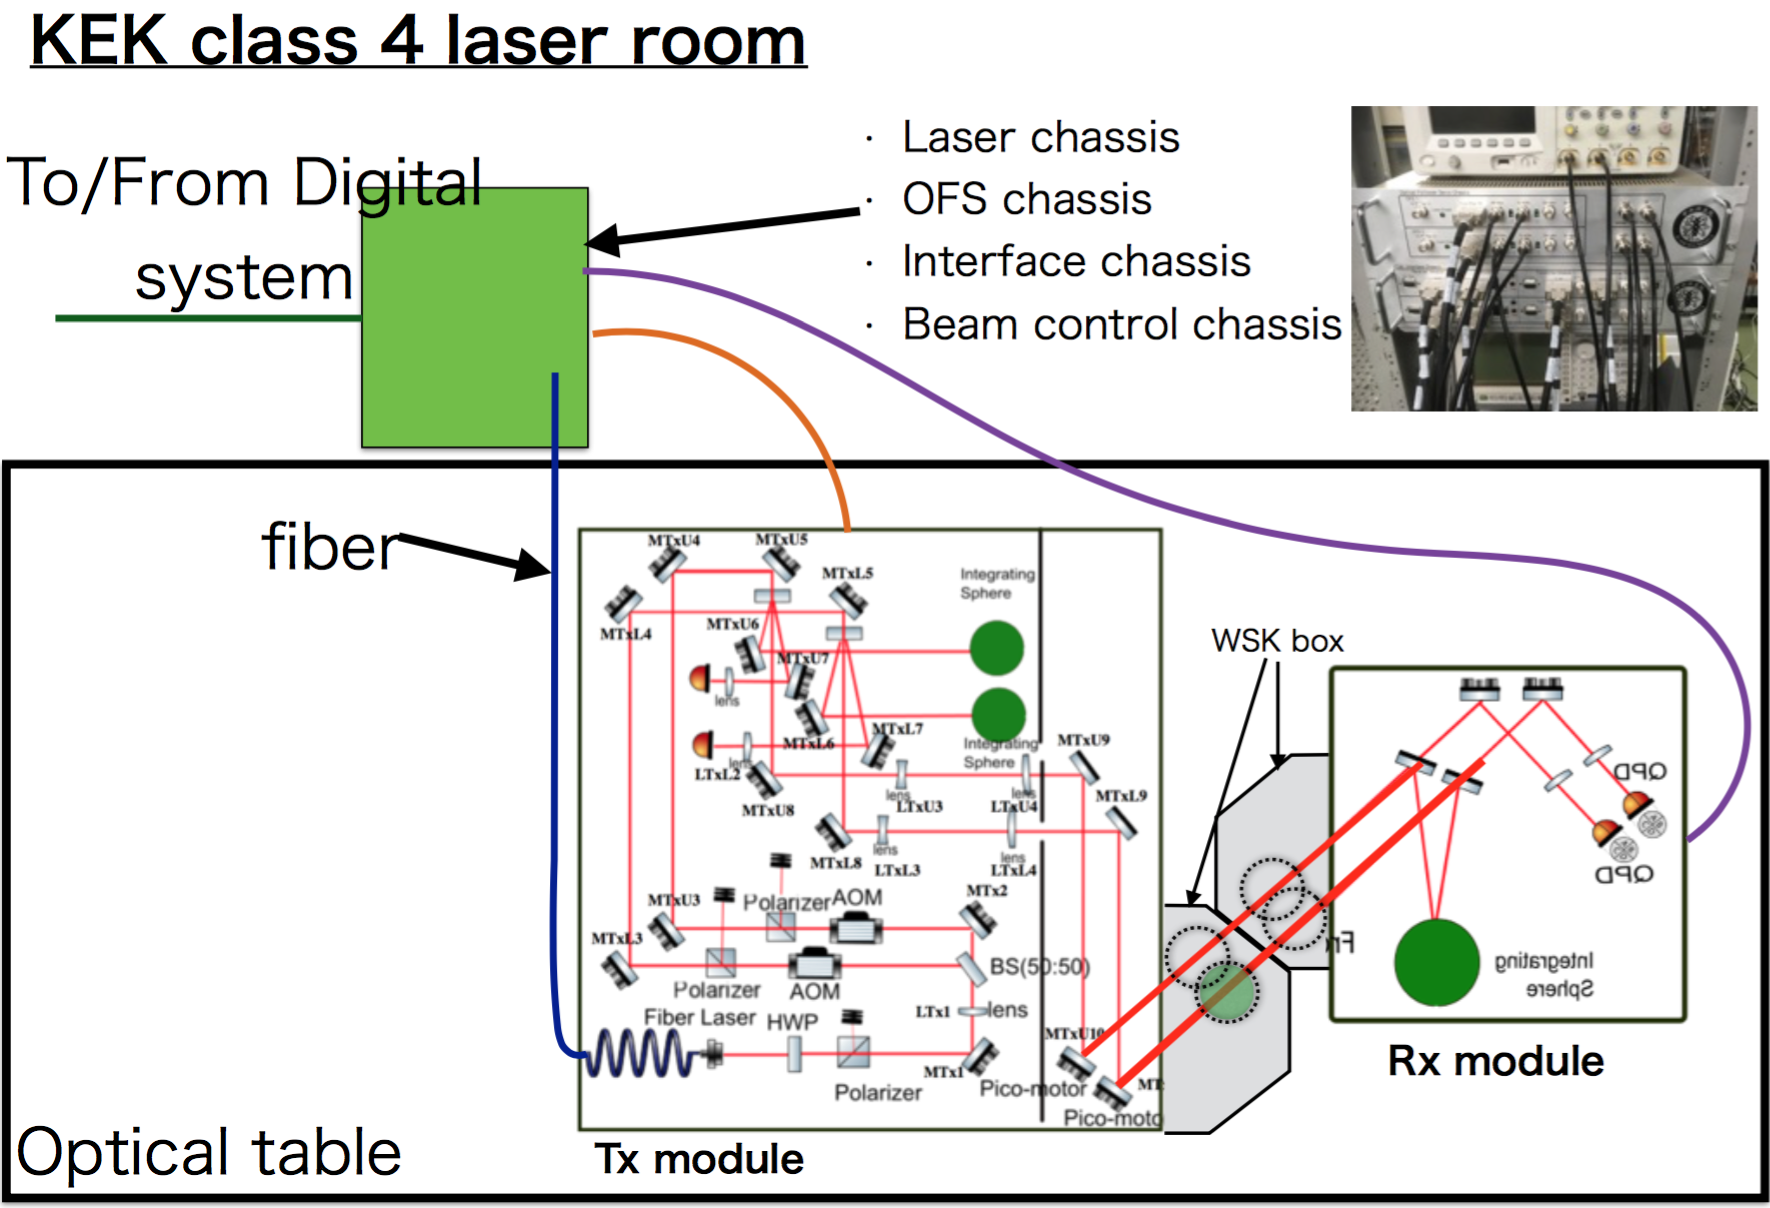
\includegraphics[width=15cm]{Setup_170109.eps}
                 \caption{Setup of the integration test} 
                 \label{fig:Setup} 
	\end{center}
\end{figure}
\subsection{Log: 01\/09}
Main goal of Jan. 9th measurement is noise debugging.
In previous measurement, the measured noise is larger than that of requirement.
To reduce the noise, we tried the following things:
\paragraph{Open loop gain}





\section{Run2 (201702; Toyama)}

\section{Run3 (201703; KAGRA Y-end)}
%----------------------------------------------------------------------------------------

